\section{Experiments}

\label{sec:experiments}

We evaluate our method on class-to-image (ImageNet), text-to-image (T2I), text-to-video (T2V), text-to-audio (T2A), and multi-modal generation. 
Through quantitative results, qualitative comparisons, and scaling experiments, we demonstrate the effectiveness of our approach, its adaptability across tasks and modalities, and its scaling properties.

% ============================================
% FIGURE: Qualitative results (t2i)
% ============================================

\begin{table}[t]
  \centering
  \caption{\textbf{Quantitative results on ImageNet 256$\times$256.} Our method outperforms REPA, despite its use of DINOv2 which heavily relies on ImageNet for training. Our method is beneficial in combination with representation autoencoders.}
  \label{tab:imagenet}
  \small
  \setlength{\tabcolsep}{3pt}
  \begin{tabular}{@{}lcccccc@{}}
    \toprule
    Model & Steps & FID$\downarrow$ & sFID$\downarrow$ & IS$\uparrow$ & Pre.$\uparrow$ & Rec.$\uparrow$ \\
    \midrule
    \multicolumn{7}{l}{\textit{Without external representations}} \\
    SiT-XL/2 & 7M & 8.3 & 6.30 & 130.57 & 0.69 & 0.67 \\
    SRA & 4M & 7.27 & 5.87 & 143.06 & 0.69 & \underline{0.68} \\
    \textbf{Ours} & {4M} & \textbf{5.70} & \textbf{4.97} & \underline{151.40} & \textbf{0.72} & {0.67} \\
    \midrule
    \multicolumn{7}{l}{\textit{With external representations}} \\
    REPA & 4M & \underline{5.89} & \underline{5.73} & \textbf{157.66} & \underline{0.70} & \textbf{0.69} \\
    \addlinespace[0.3em]
    \hdashline
    \addlinespace[0.3em]
    \multicolumn{6}{l}{\textit{With representation autoencoders}} \\
    RAE & 1M & 3.24 & 6.73 & 218.53 & 0.83 & 0.54 \\
    RAE + Ours & 1M & \textbf{2.95} & \textbf{5.50} & \textbf{222.34} & \textbf{0.84} & \textbf{0.56} \\
    \bottomrule
  \end{tabular}
\end{table}

\begin{figure}[t]
    \centering
    \begin{subfigure}[t]{0.49\linewidth}
      \centering
      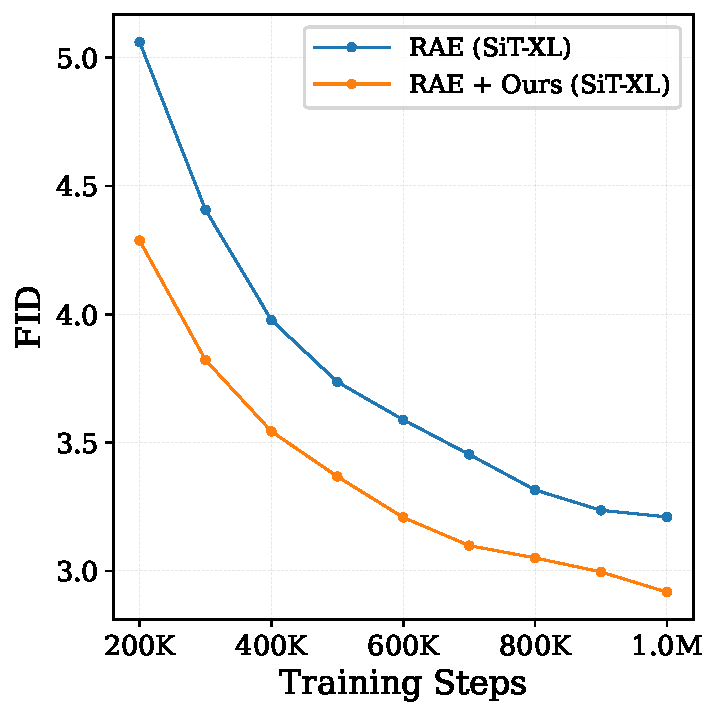
\includegraphics[width=\linewidth]{figures/RAE_v3.pdf}
      \caption{Our method w/ RAE}
      \label{fig:imagenet_RAE}
    \end{subfigure}
    \hfill
    \begin{subfigure}[t]{0.49\linewidth}
      \centering
      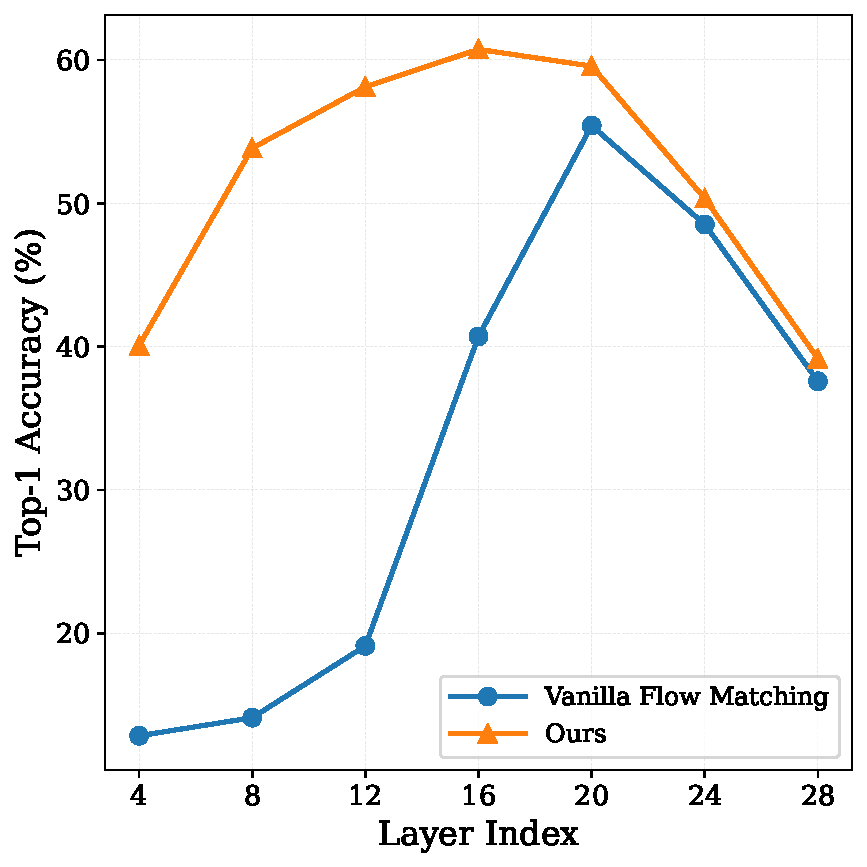
\includegraphics[width=\linewidth]{figures/linear_probe_accuracy.pdf}
      \caption{Linear probing on ImageNet}
      \label{fig:linear_prob}
    \end{subfigure}
    \caption{\textbf{Autoencoder generalization and improved representations.} (a) Our method improves training and generation in RAE~\citep{rae}, demonstrating compatibility with semantic latent spaces. (b) Linear probing confirms that our method learns stronger representations than standard flow matching.}
    \label{fig:additional_imagenet}
    \vspace{-10px}
\end{figure}

\begin{table*}[t]
  \begin{minipage}[t]{0.58\textwidth}
    \centering
    \captionof{table}{\textbf{Quantitative results on text-to-image generation.} Our method outperforms all external and internal alignment methods.}
    \label{tab:t2i}
    \small
    \setlength{\tabcolsep}{2.5pt}
    \begin{tabular}{@{}lccccccccc@{}}
      \toprule
      Model & Steps & FID$\downarrow$ & sFID$\downarrow$ & IS$\uparrow$ & Pre.$\uparrow$ & Rec.$\uparrow$ & FD-DINO$\downarrow$ & CLIP$\uparrow$ \\
      \midrule
      \multicolumn{9}{l}{\textit{Without external representations}} \\
      Vanilla Flow & 1M & 4.08 & 8.16 & 20.49 & 0.62 & \underline{0.64} & 204.49 & 30.66 \\
      SRA & 1M & \underline{3.70} & \textbf{8.05} & 21.00 & \underline{0.63} & \underline{0.64} & 176.79 & \underline{30.78} \\
      \textbf{Ours} & {1M} & \textbf{3.61} & 8.14 & \textbf{21.19} & \textbf{0.64} & \textbf{0.65} & \textbf{167.98} & \textbf{30.88} \\
      \midrule
      \multicolumn{9}{l}{\textit{With external representations}} \\
      REPA & 1M & 3.92 & 8.20 & \underline{21.16} & \underline{0.63} & \textbf{0.65} & \underline{173.35} & 30.67 \\
      SigLIP 2 & 1M & 3.97 & \underline{8.13} & 20.65 & \underline{0.63} & \underline{0.64} & 196.75 & 30.68 \\
      \bottomrule
    \end{tabular}
  \end{minipage}
  \hfill
  \begin{minipage}[t]{0.40\textwidth}
    \centering
    \captionof{table}{\textbf{Quantitative results on video generation.} Most external models harm performance.}
    \label{tab:video}
    \small
    \setlength{\tabcolsep}{5pt}
    \begin{tabular}{@{}lccc@{}}
      \toprule
      Model & Steps & FVD$\downarrow$ & FID$\downarrow$ \\
      \midrule
      \multicolumn{4}{@{}l}{\textit{Without external representations}} \\
      Vanilla Flow & 600K & 50.95 & 9.28 \\
      SRA & 600K & 49.75 & \underline{9.02} \\
      \textbf{Ours} & 600K & \textbf{47.81} & \textbf{8.92} \\
      \midrule
      \multicolumn{4}{@{}l}{\textit{With external representations}} \\
      w/ DINOv2 & 600K & \underline{49.59} & 9.39 \\
      w/ Depth Anything 3 & 600K & 51.52 & 9.85 \\
      w/ V-JEPA2 & 600K & 53.55 & 9.91 \\
      \bottomrule
    \end{tabular}
  \end{minipage}
  % \vspace{-6px}
\end{table*}

\begin{table}[t]
    \caption{\textbf{Quantitative results on audio generation.} 
    Our method achieves the best FAD scores across multiple CLAP variants.
    }
\label{tab:audio}
\centering
\small
\setlength{\tabcolsep}{5pt}
\begin{tabular}{@{}lcccc@{}}
\toprule
Model & Steps & CLAP$\downarrow$ & CLAP-M$\downarrow$ & CLAP-A$\downarrow$ \\
\midrule
\multicolumn{5}{@{}l}{\textit{Without external representations}} \\
    Vanilla Flow & 350K & 148.874 & 0.1695 & 0.1059 \\
    SRA & 350K & \underline{147.215} & \underline{0.1664} & \underline{0.1034} \\
    \textbf{Ours} & 350K & \textbf{145.645} & \textbf{0.1634} & \textbf{0.1001} \\
\midrule
\multicolumn{5}{@{}l}{\textit{With external representations}} \\
    w/ MERT & 350K & 148.883 & 0.1677 & 0.1040 \\
\bottomrule
\end{tabular}
\vspace{-12px}
\end{table}

\begin{figure*}[t]
  \centering
  
  \begin{subfigure}[t]{0.245\textwidth}
    \centering
    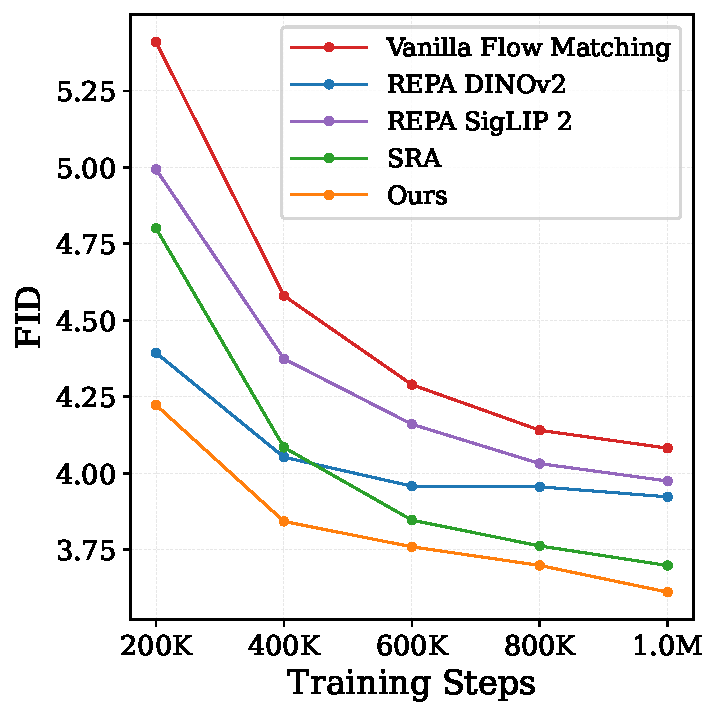
\includegraphics[width=\linewidth]{figures/t2i_fid.pdf}
    \caption{T2I FID$\downarrow$}
    \label{fig:t2i_fid}
  \end{subfigure}%
  \hfill%
  \begin{subfigure}[t]{0.245\textwidth}
    \centering
    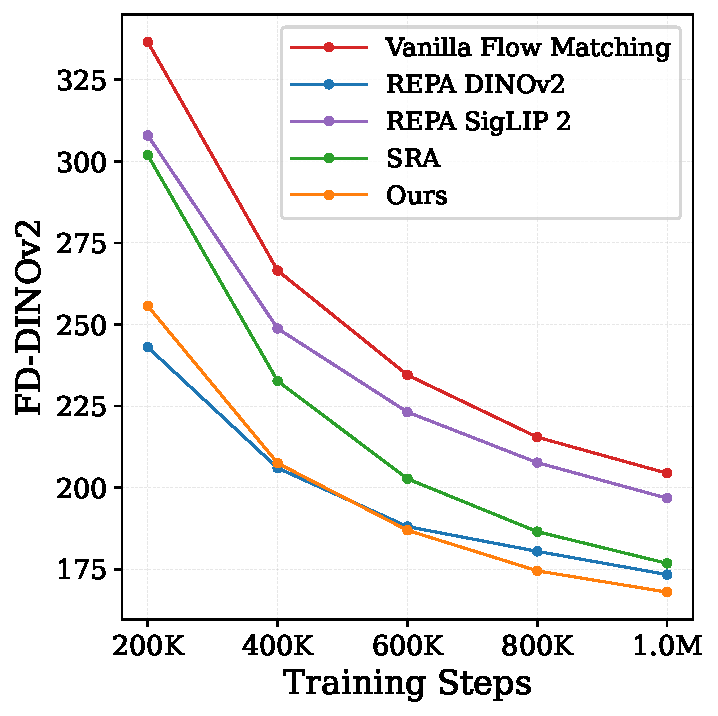
\includegraphics[width=\linewidth]{figures/fd_figure.pdf}
    \caption{T2I FD-DINOv2$\downarrow$}
    \label{fig:results_t2i_fid}
  \end{subfigure}%
  \hfill%
  \begin{subfigure}[t]{0.245\textwidth}
    \centering
    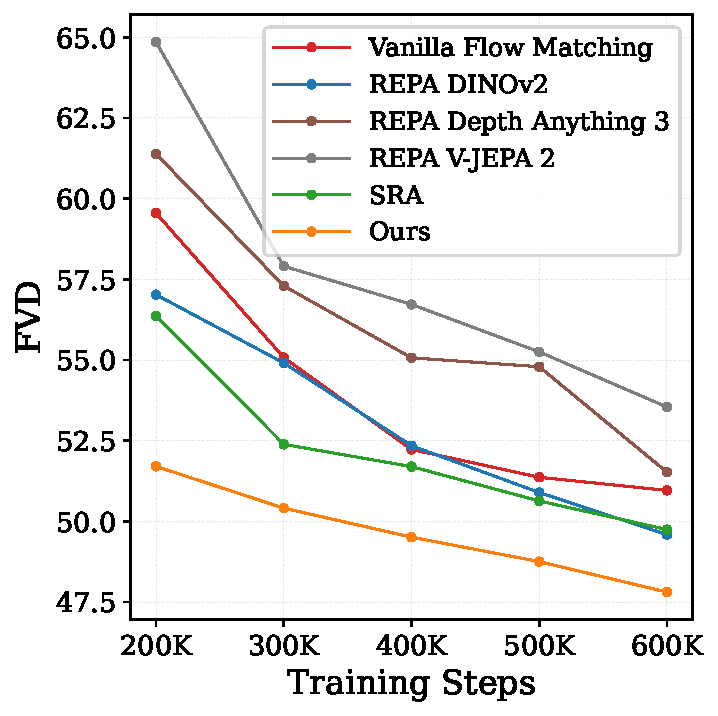
\includegraphics[width=\linewidth]{figures/fvd_figure.pdf}
    \caption{Video FVD$\downarrow$}
    \label{fig:results_video_fvd}
  \end{subfigure}%
  \hfill%
  \begin{subfigure}[t]{0.245\textwidth}
    \centering
    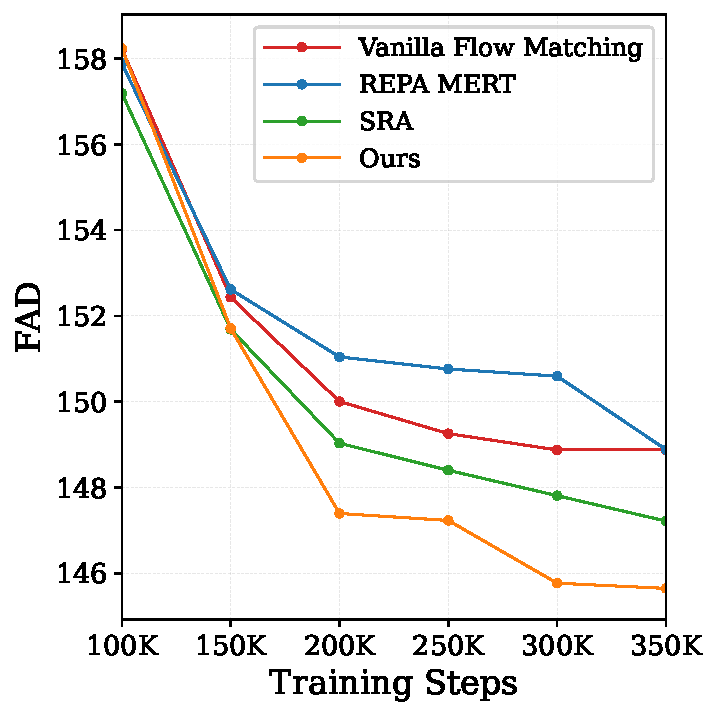
\includegraphics[width=\linewidth]{figures/fad_clap_ms.pdf}
    \caption{Audio FAD$\downarrow$}
    \label{fig:results_audio_fad}
  \end{subfigure}
  
  \caption{\textbf{Quantitative results across modalities.} Our method significantly outperforms all external and internal alignment methods across text-based image, video, and audio generation. Our method is the only one to outperform REPA on DINOv2 FD (despite REPA directly aligning with DINOv2). Arrows indicate whether lower ($\downarrow$) or higher ($\uparrow$) is better.}
  \label{fig:quantitative_results}
\end{figure*}
  
\textbf{Implementation Details.} 
For ImageNet experiments, we use SiT-XL~\cite{sit} with the REPA setup. All other experiments use the FLUX.2~\cite{bfl2025representation} transformer with domain-specific autoencoders. Unless noted, all models are $\sim$625M parameters. For text-to-image (T2I), we use the Stable Diffusion autoencoder (following the ImageNet setup) and train on 20M text-image pairs; for text-to-video (T2V), the Wan2.2~\cite{wan2025} autoencoder with 6M videos; for text-to-audio (T2A), the Songbloom autoencoder~\cite{yang2025songbloom} with FMA~\citep{fma_dataset}. All evaluations are conducted on holdout sets of the corresponding training sets. See App.~\ref{app:implementation} for further training and sampling details.

\subsection{Single Modality Experiments}
\label{subsec:singlemodality}

\textbf{Baselines.} We compare against vanilla flow matching and the leading methods from both categories of representation alignment: with and without external models. For each category, we select the best performing approach applicable across all tested modalities: REPA~\citep{repa} for external alignment and SRA~\citep{sra} for methods without external models (see App.~\ref{suppsec:layersync}). To ensure a thorough comparison, we additionally evaluate external encoders that are, in theory, better suited than DINO to each task: SigLIP 2~\citep{siglip2} for text-to-image (trained with text supervision and multi-aspect ratio support), V-JEPA 2~\citep{bardes2024vjepa} and Depth Anything 3~\citep{da3} for video, and MERT~\citep{li2024mertacousticmusicunderstanding} for audio. 

\textbf{Quantitative Results.}
On ImageNet (Tab.~\ref{tab:imagenet}), our method outperforms REPA (FID 5.70 vs 5.89) without external representations and despite REPA using DINOv2, itself heavily trained on ImageNet. To our knowledge, we are the first to show self-supervised learning outperforming external alignment on ImageNet.
To demonstrate generalization to arbitrary latent spaces, we apply our method to 
RAE~\cite{rae}, in the same setup as the other experiments. As shown in Fig.~\ref{fig:imagenet_RAE} and Tab.~\ref{tab:imagenet}, this yields significant improvements (FID 3.24 → 2.95).
See App.~\ref{sec:RAE} for further details. Finally, Fig.~\ref{fig:linear_prob} shows linear probing results after 2M training steps. Our method significantly boosts the representation quality of early and mid layers, confirming that representations improve alongside generations.

On the T2I task (Fig.~\ref{fig:quantitative_results}a,b, Tab.~\ref{tab:t2i}), our method achieves the best FID (3.61) among all methods, outperforming both external alignment approaches (REPA: 3.92, SigLIP 2: 3.97) and methods without external models (SRA: 3.70). Notably, we outperform REPA even when computing the Fr\'echet distance score with DINOv2 features (Fig.~\ref{fig:quantitative_results}b, 167.98 vs 173.35) despite REPA explicitly aligning with DINOv2 features, a gap no other baseline closes. Our method also achieves the highest CLIP score, indicating superior text-image alignment.

\enlargethispage{\baselineskip}
Our approach shows particularly strong gains on \emph{video generation} (Fig.~\ref{fig:quantitative_results}c, Tab.~\ref{tab:video}), achieving the best FVD (47.81) and FID (8.92, per frame) by a significant margin; the next best method (REPA) trails by nearly 2 FVD points. Notably, external alignment with video-specific V-JEPA2~\citep{bardes2024vjepa} and Depth Anything 3~\citep{da3} actually \emph{harms} performance relative to vanilla flow matching. We hypothesize that temporal relations are harder to learn than spatial ones, making objective misalignments harder to bridge. Moreover, video temporal redundancies allow models to exploit shortcuts by copying across frames rather than learning meaningful semantics, a behavior our masking mechanism naturally discourages.

We observe similar trends for audio (Fig.~\ref{fig:quantitative_results}d, Tab.~\ref{tab:audio}): our method achieves the best FAD scores across all CLAP variants, while external alignment with MERT provides no benefit over vanilla flow matching. This is further indication that external alignment struggles to generalize.

\begin{figure}[t]
    \centering
    \begin{subfigure}[t]{0.495\linewidth}
      \centering
      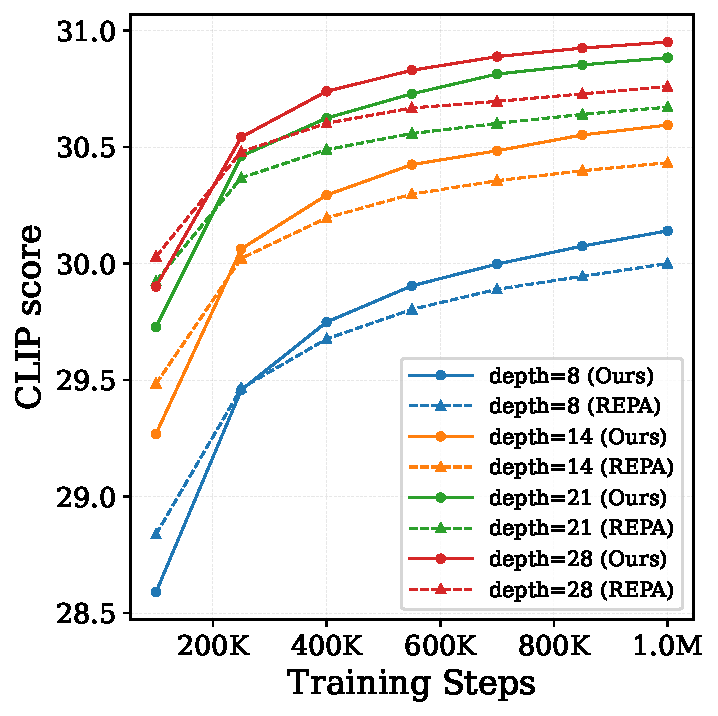
\includegraphics[width=\linewidth]{figures/scaling_clip_score_v5.pdf}
      \caption{Steps}
      \label{fig:scaling_steps}
    \end{subfigure}
    \hfill
    \begin{subfigure}[t]{0.495\linewidth}
      \centering
      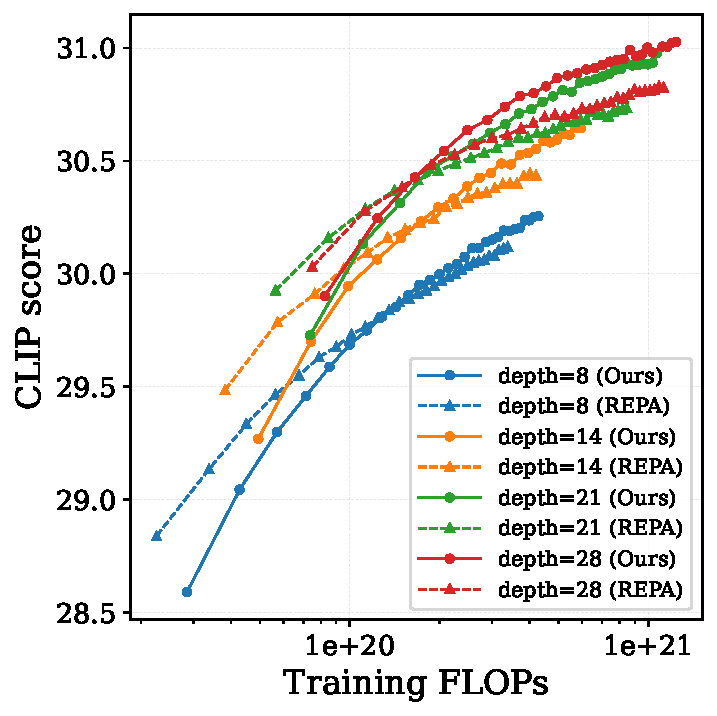
\includegraphics[width=\linewidth]{figures/scaling_flops_v4.pdf}
      \caption{FLOPs}
      \label{fig:scaling_flops}
    \end{subfigure}
    \caption{\textbf{Scaling behavior.} As model size increases (290M → 420M → 625M → 1B parameters), the performance gap between our method and REPA widens (a). Notably, our 625M variant outperforms the 1B REPA model. Our method effectively leverages increased compute, while REPA shows diminishing returns (b).}
    \label{fig:scaling}
    \vspace{-12px}
\end{figure}

\textbf{Scaling Behavior.} 
We evaluate the scaling behavior of our method and REPA by training text-to-image models at four scales: 290M (deph=8), 420M (depth=14), 625M (depth=21), and 1B (depth=28).
Fig.~\ref{fig:scaling_steps} shows that as we scale the model, the performance gap between our method and REPA widens consistently in our favor. Notably, our 625M parameter model outperforms the 1B REPA model, demonstrating the significant performance gains from our approach at scale. Fig.~\ref{fig:scaling_flops} demonstrates that our method exhibits consistent improvements with increased compute, following expected scaling laws. These results validate our hypothesis that tying the model to a fixed external encoder creates a bottleneck that limits the benefits of scaling, whereas our unified framework scales as expected.

\begin{figure*}[t]
  \centering
      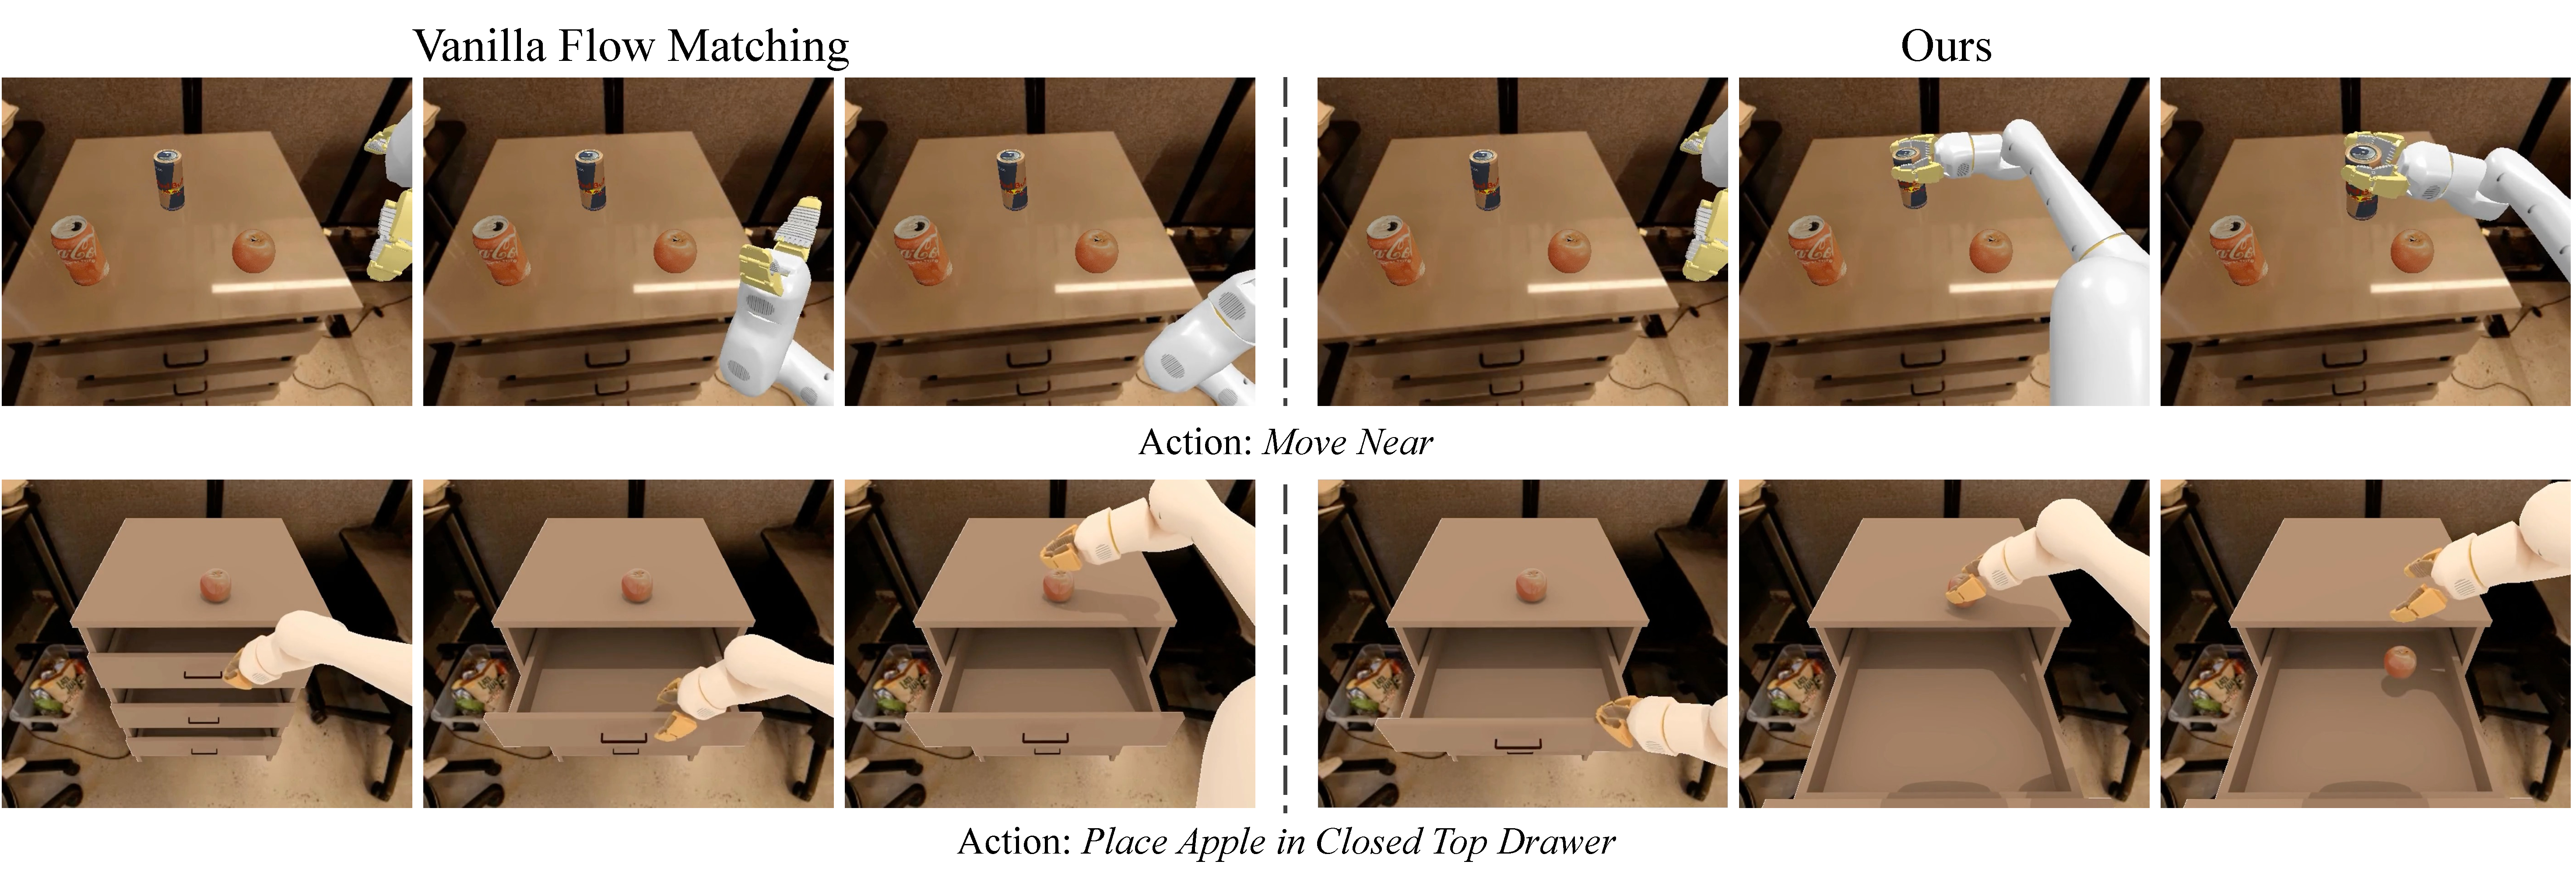
\includegraphics[width=\linewidth]{figures/simpler.pdf}
      \vspace{-18px}
    \caption{\textbf{SIMPLER simulation rollouts.} Our method significantly boosts success rate for complex actions such as Move Near (top) and Open and Place (bottom).}
  \label{fig:robotics}
  \vspace{-12px}
\end{figure*}

\begin{figure}[t]
  \centering
  \begin{subfigure}[t]{0.25\textwidth}
      \centering
      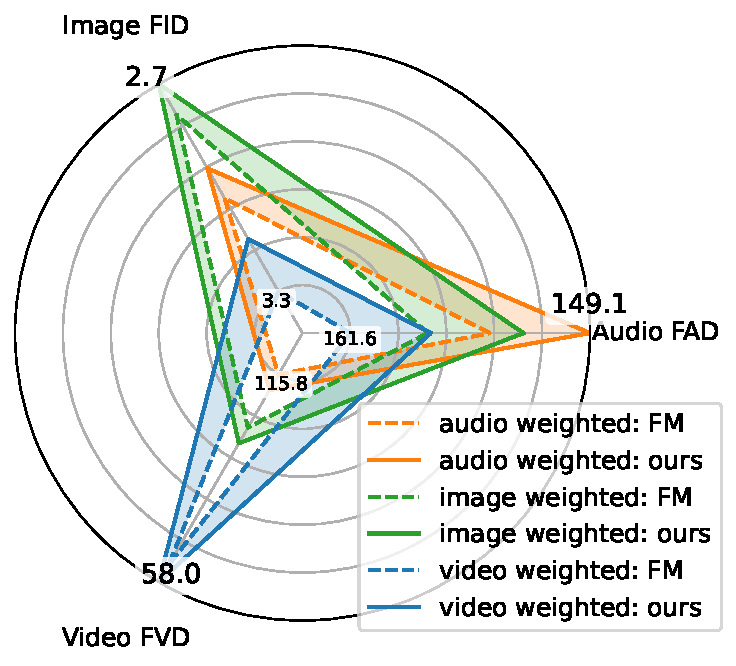
\includegraphics[width=\linewidth]{figures/mixed/radar.pdf}
    \caption{Multi-Modal Training}
    \label{fig:audio_mixed}
  \end{subfigure}%
  \begin{subfigure}[t]{0.25\textwidth}
    \centering
    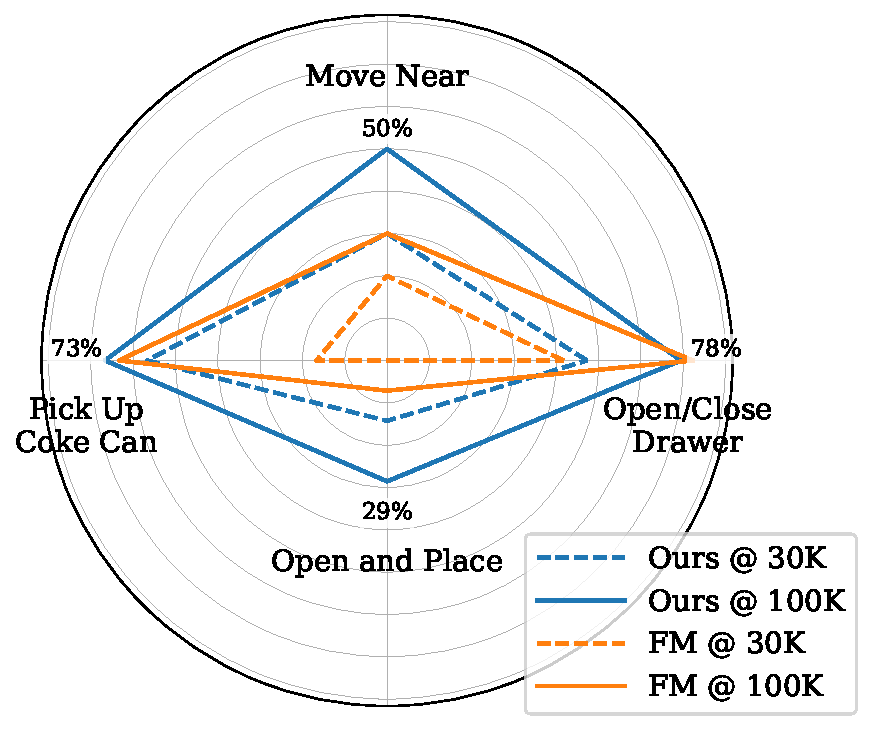
\includegraphics[width=\linewidth]{figures/action/radar_plot_main.pdf}
    \caption{Joint Video-Action Training}
    \label{fig:results_joint}
  \end{subfigure}
    \caption{\textbf{Multi-modal experiments.} (a) We train a single model on three modalities with different weightings to control the trade-off between them. Ours provides consistent improvements (shaded area) across all settings. Axes are inverted so that larger area indicates better performance. (b) Success rates for joint Video-Action prediction. Early on (30k), Ours outperforms FM across all tasks and achieves success in all task categories, whereas FM fails entirely on Open and Place tasks. Later (100k), performance on single-object tasks (Pick Coke Can, Open/Close Drawer) converges, while Ours maintains a significant advantage on complex multi-object and sequential tasks (Move Near, Open and Place).}
  \label{fig:mixed_quantitative_results}
  \vspace{-12px}
\end{figure}

\begin{table*}[t!]
  \centering
  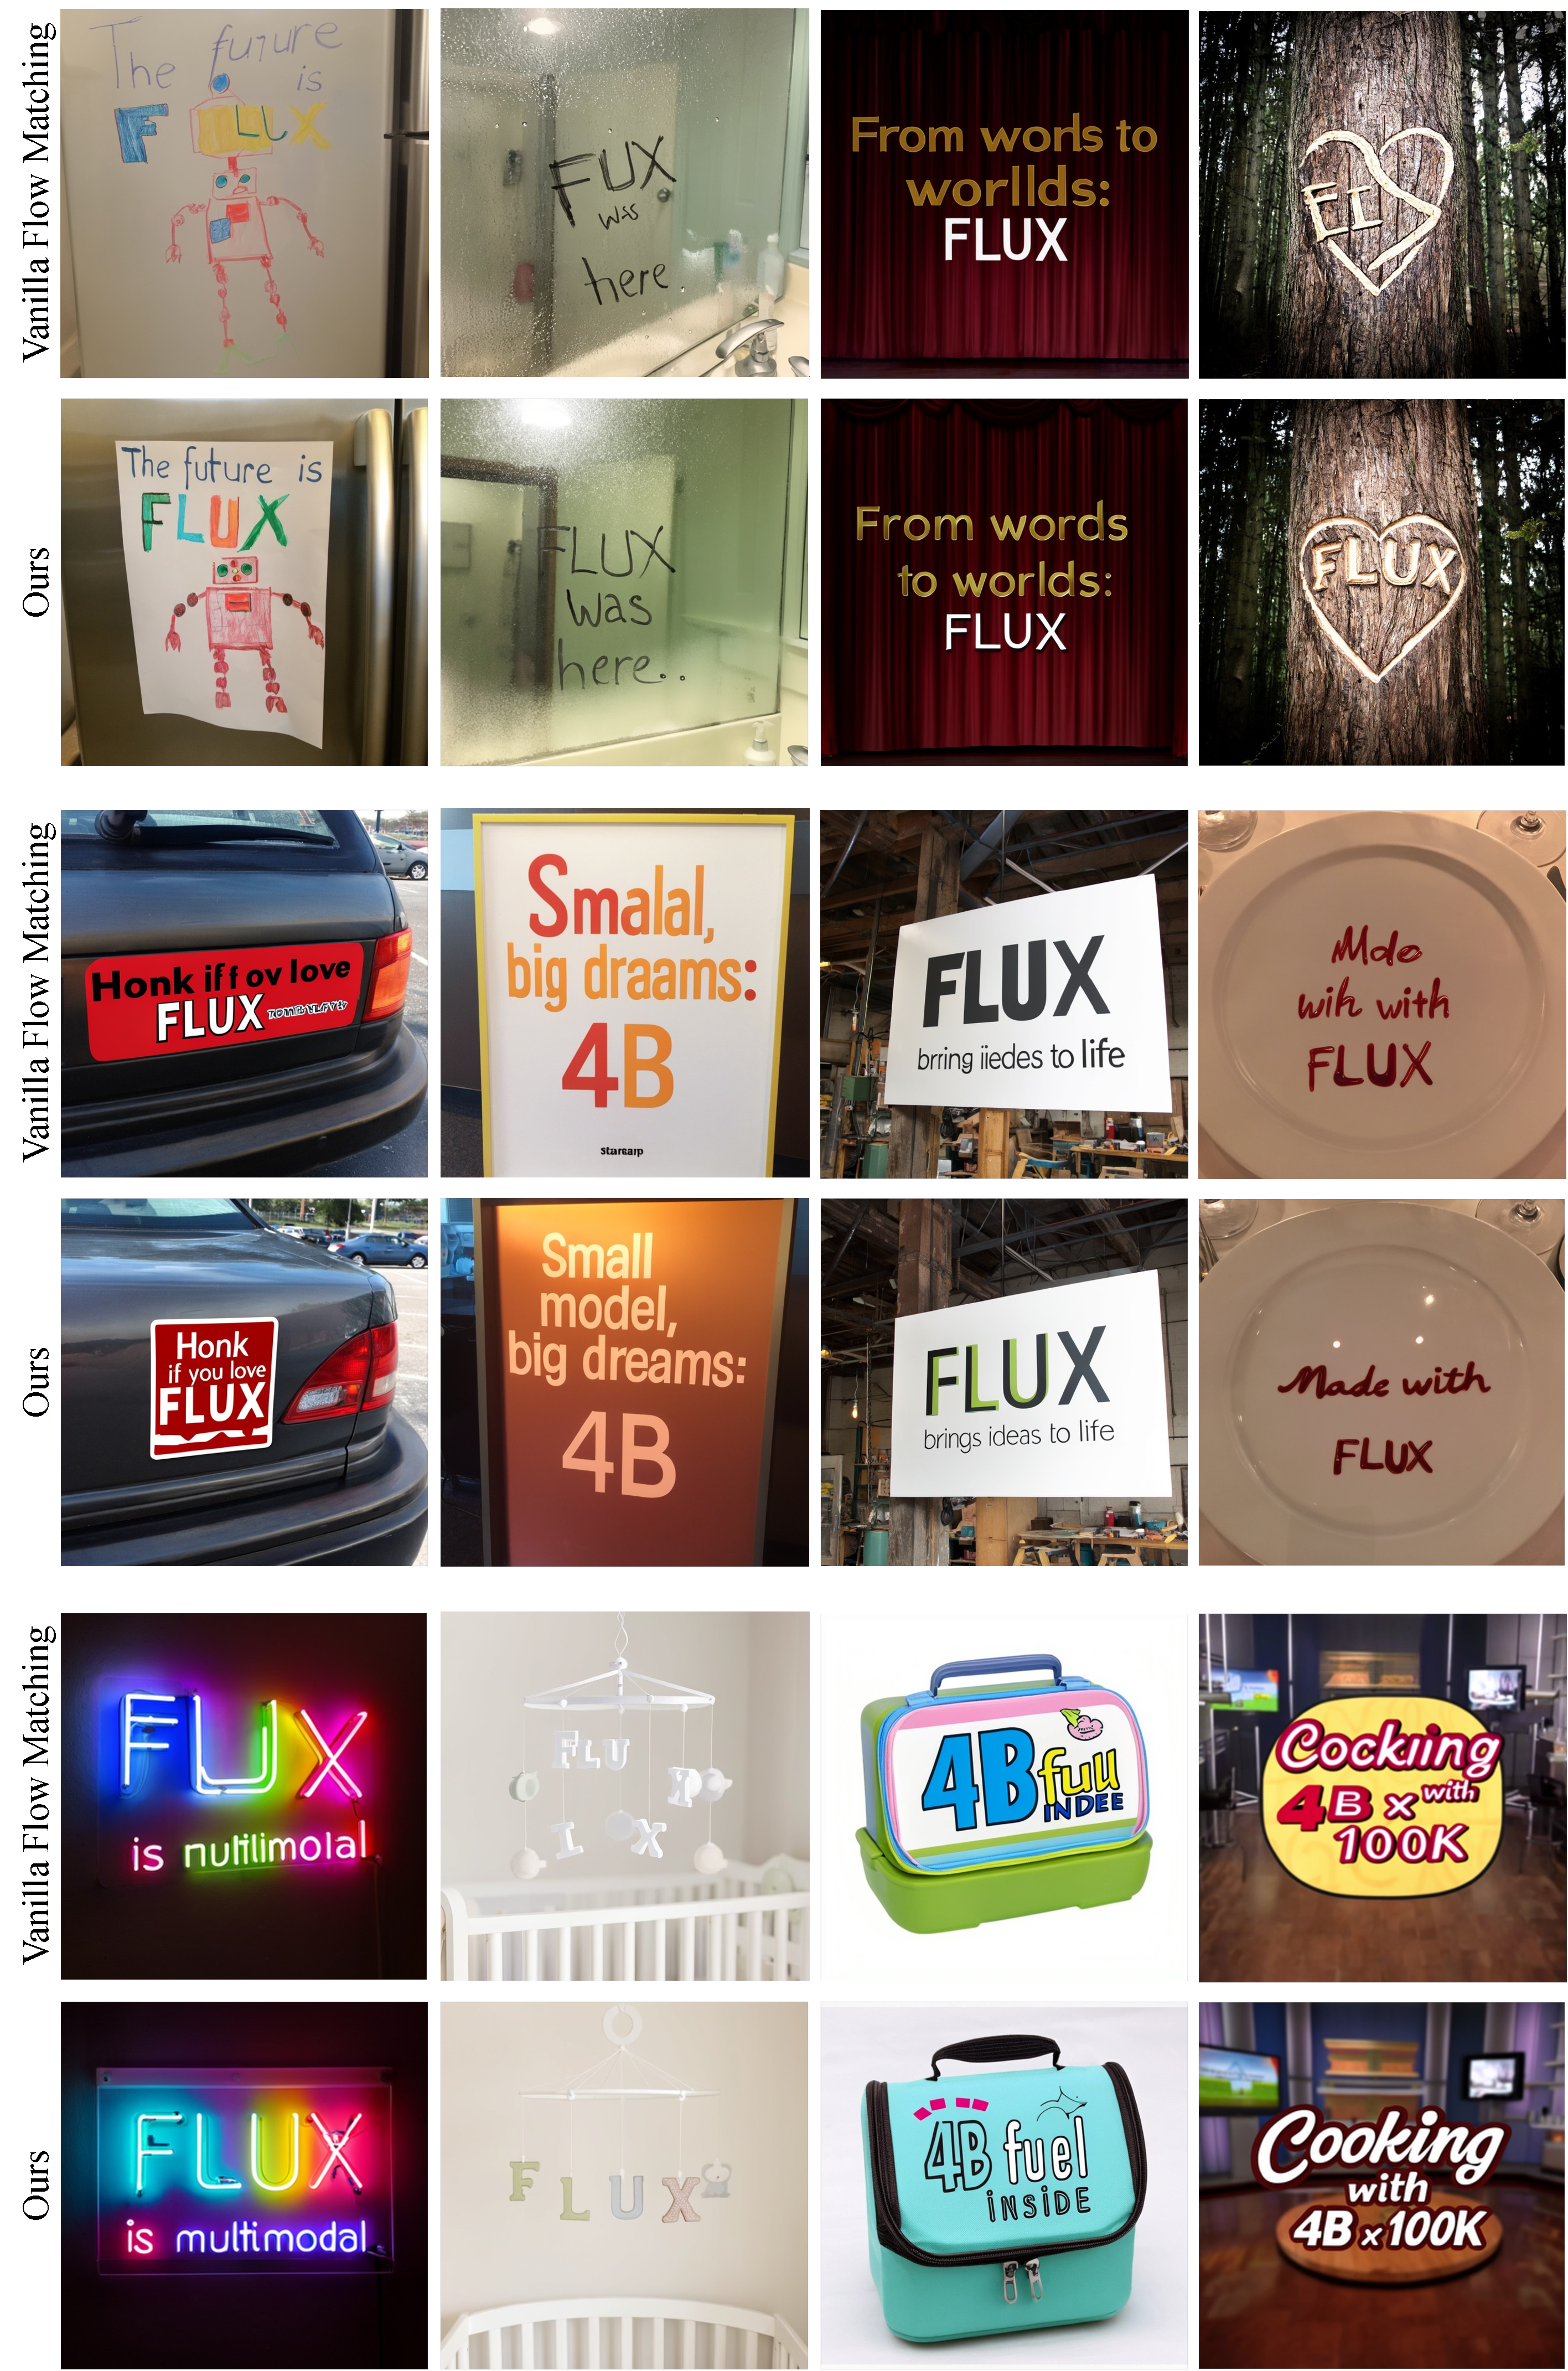
\includegraphics[width=0.87\linewidth]{figures/flux_typo.pdf}
  \captionof{figure}{\textbf{Typography comparison.} 
  Self-Flow significantly outperforms standard flow matching in accurate text rendering.}
  \label{fig:text_rendering}
  \vspace{-10px}
\end{table*}

\begin{figure*}[t!]
  \centering
  \begin{subfigure}[t]{\linewidth}
    \centering
    \includegraphics[width=0.99\linewidth]{figures/t2i.pdf}
    \vspace{-4px}
    \caption{\textbf{Text-to-image.} Our method produces superior structure, texture, and fine-grained details across prompts of varying complexity.}
    \label{fig:qualitative_image}
  \end{subfigure}
  
  
  \begin{subfigure}[H]{\linewidth}
    \centering
    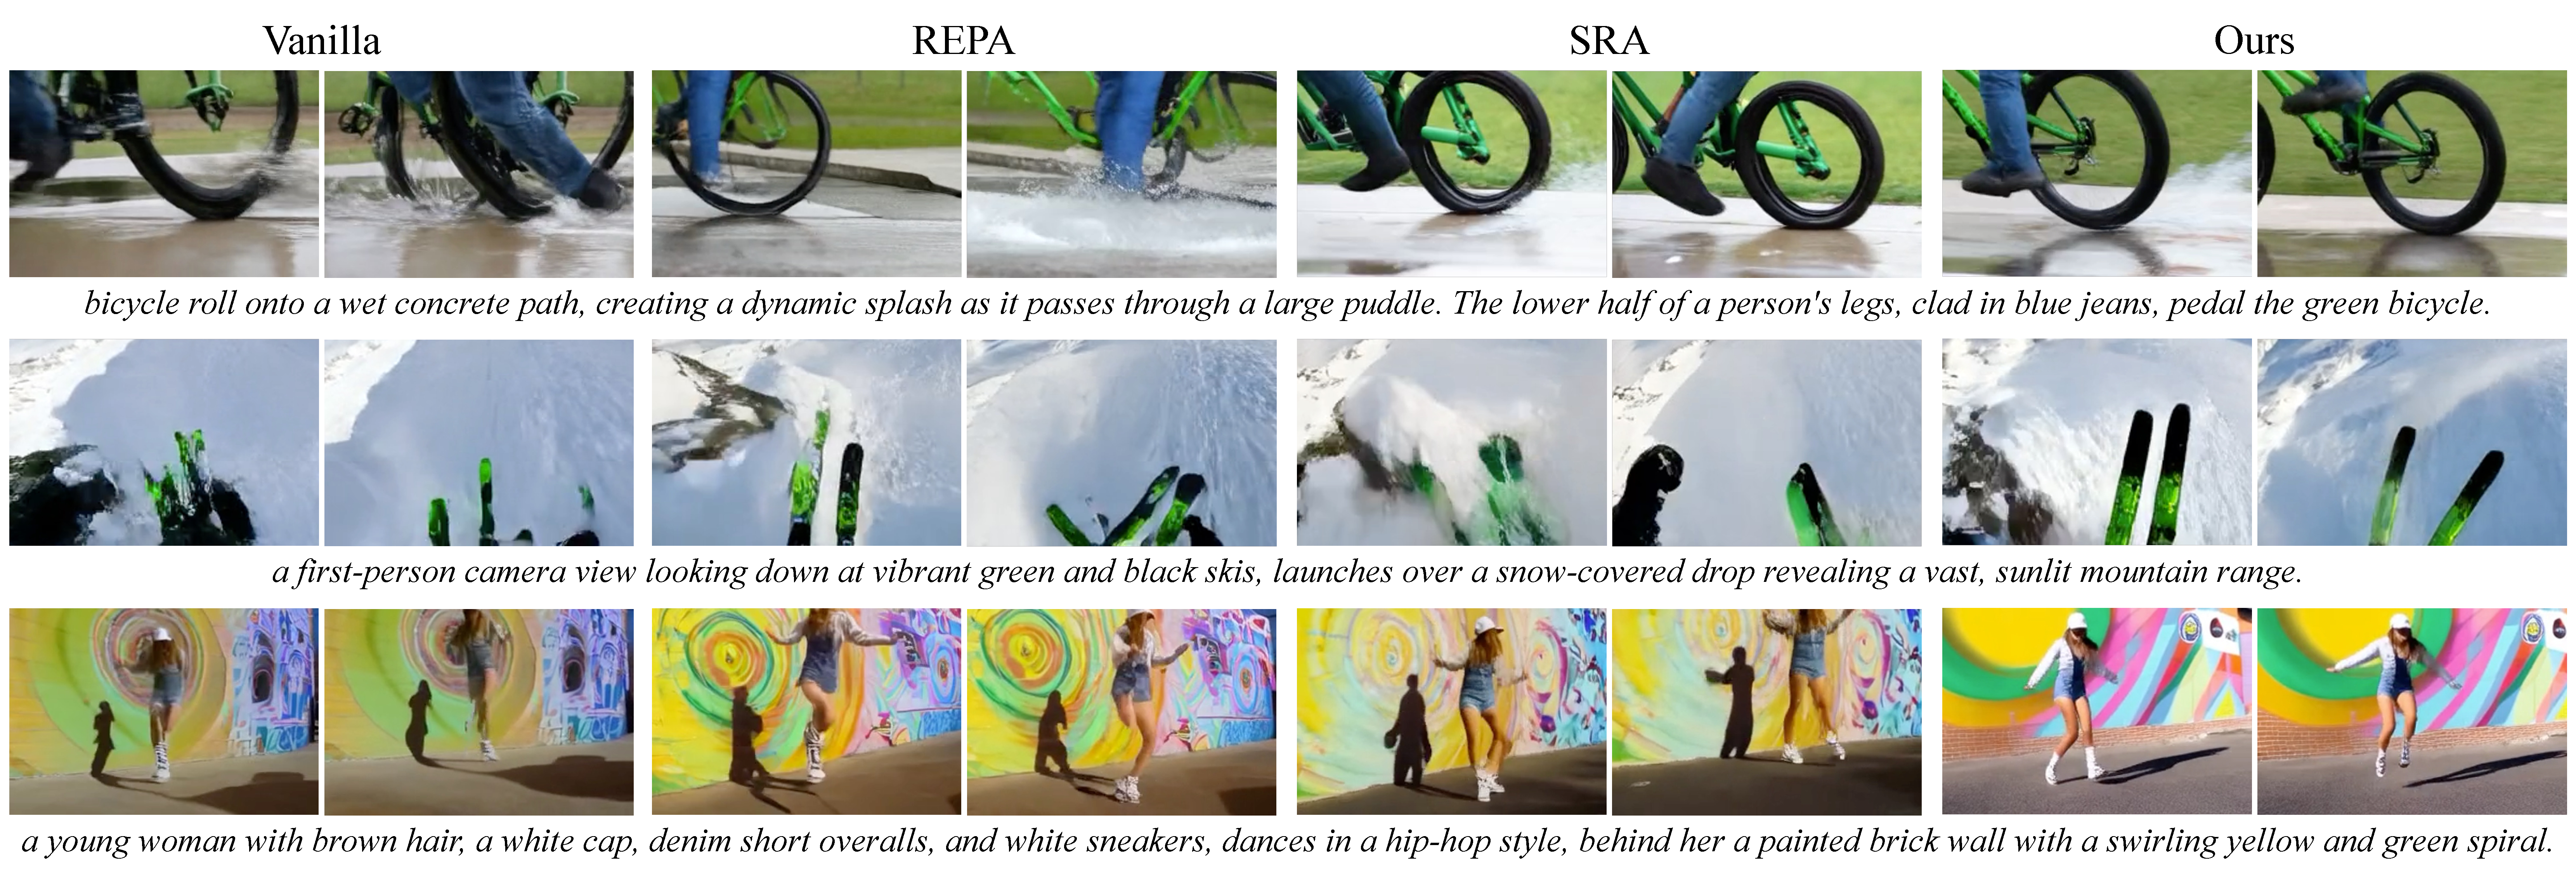
\includegraphics[width=\linewidth]{figures/t2v.pdf}
    \vspace{-12px}
    \caption{\textbf{Text-to-video.} Baselines exhibit structural and temporal artifacts, while our method produces coherent and temporally smooth results.}
    \label{fig:qualitative_video}
  \end{subfigure}
  \vspace{-2px}
  \caption{\textbf{Qualitative comparisons} with vanilla flow matching and leading baselines: external (REPA) and internal (SRA). \vspace{-0.5em}}
  \label{fig:qualitative}
  \vspace{-2px}
\end{figure*}

\begin{figure}[t]
    \centering
    \begin{subfigure}[t]{0.495\linewidth}
      \centering
      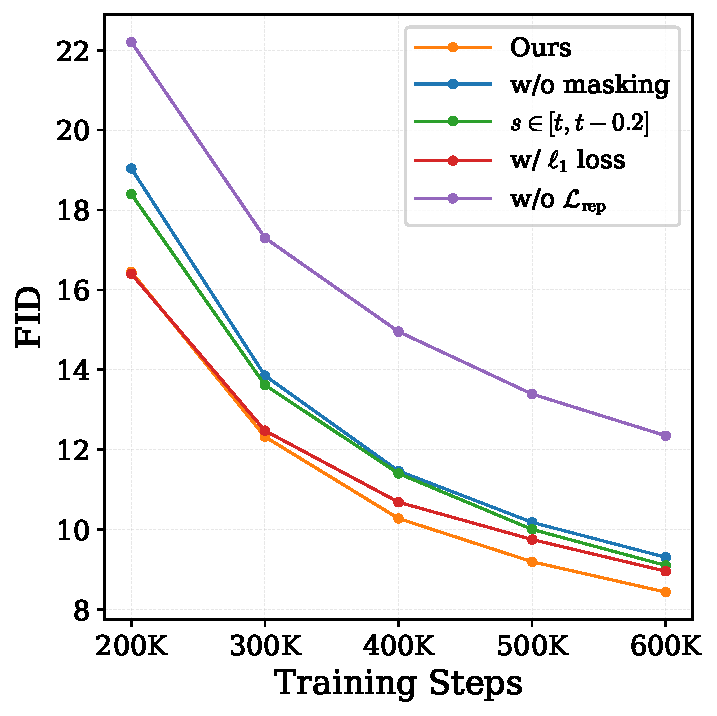
\includegraphics[width=\linewidth]{figures/ablation_figure.pdf}
      \caption{Ablation study}
      \label{fig:ablations}
    \end{subfigure}
    \hfill
    \begin{subfigure}[t]{0.495\linewidth}
      \centering
      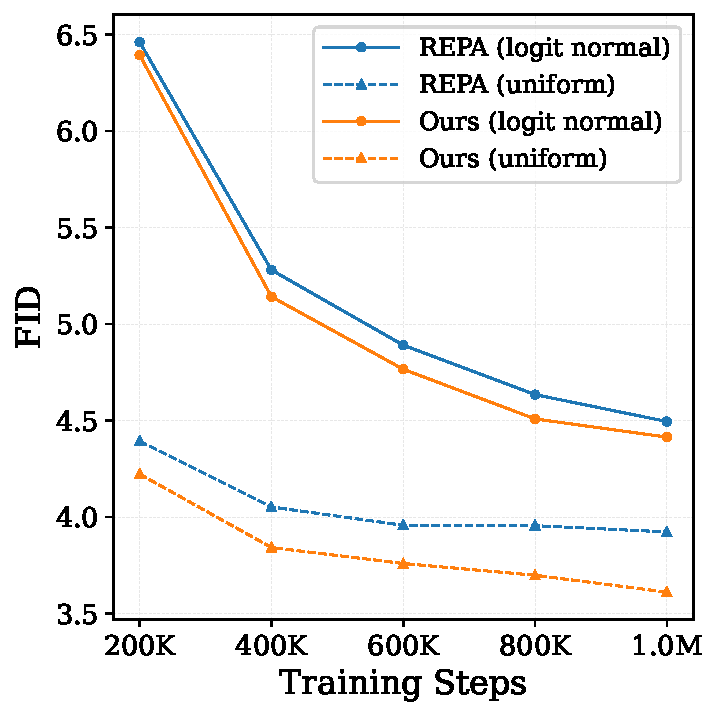
\includegraphics[width=\linewidth]{figures/noise_scheduler_impact.pdf}
      \caption{Impact of noise scheduler}
      \label{fig:limitations}
    \end{subfigure}
    \caption{\textbf{Ablations and Limitations.} (a) Removing the self-supervised loss is most detrimental. Removing Dual-Timestep Scheduling or changing the scheduling of the second timestep ($s$) significantly harms the results. (b) While better noise scheduling impacts both methods positively, our method benefits from it more. \vspace{-2em}}
    \label{fig:ablations_limitations}
    \vspace{-4px}
\end{figure}


\subsection{Multi-Modal Experiments}
\label{subsec:multimodal}
Having established the benefits of our approach on individual modalities, we now explore mixed and joint multi-modal setups. The former refers to a single model trained on multiple modalities, the latter to simultaneous generation of multi-modal outputs (e.g., video and corresponding audio or actions for robotic embodiments).

For the mixed-modality experiments, we follow the single-modality setup, except that we use the FLUX.2 autoencoder for T2I for enhanced visual quality. To systematically test our method's impact on each modality within this mixed setting, we employ modality-specific loss weightings $w=(w_I>0,w_V>0,w_A>0)$, taking into consideration the number of samples observed for each modality (additional details in App.~\ref{app:implementation}). 
The overall loss at each step is a weighted-linear combination of each modality's loss, parameterized by $w$. A robust representation learning framework should yield improvements across all selections of $w$, demonstrating the method's ability to harmonize different representations under a single backbone. This requirement is particularly challenging due to the different nature of the modalities---while audio representations are temporal and relatively low-dimensional, video data is high-dimensional and contains significant spatial and temporal redundancies. Fig.~\ref{fig:audio_mixed} shows results in a normalized radar chart with inverted axes, using the extreme weightings that favor each modality. This allows us to test the trade-off between different modalities. Our approach consistently improves performance across all three modalities simultaneously, even under extreme setups that favor a specific modality.

Next, we consider joint video-action prediction for embodied AI, where the model jointly predicts future video frames and robot actions from a conditioning image. We initialize from the video-weighted mixed-modality model and finetune on the RT-1 robotics dataset~\citep{rt1} (73.5k episodes), evaluating on the SIMPLER simulator~\citep{simpler}. We compare Self-Flow (Ours) and vanilla flow matching (FM) initializations, both finetuned under identical conditions.
Fig.~\ref{fig:results_joint} reports the success rate by task group. Self-Flow consistently outperforms flow matching throughout finetuning, demonstrating more efficient learning from limited robotics data. Notably, while performance on single-object tasks (Pick, Open/Close) converges between methods, Self-Flow maintains a significant advantage on complex multi-object and sequential tasks (Move Near, Open and Place, see also Fig.~\ref{fig:robotics}), suggesting that our approach learns representations that improve complex visual reasoning. See App.~\ref{suppsec:action} for details on this task and App.~\ref{suppsec:videoaudio} for experiments on joint video-audio prediction.

\subsection{Qualitative Results.}
We provide qualitative comparisons in Figs.~\ref{fig:text_rendering},~\ref{fig:qualitative}, with additional results in the appendices (T2I: Figs.~\ref{fig:qualitative_image_supp}--\ref{fig:qualitative_image_supp5},~\ref{fig:text}--\ref{fig:text2}; T2V: Figs.~\ref{fig:qualitative_video_supp}--\ref{fig:qualitative_video_supp5}) and on our supplementary website, which contains the full video results and audio comparisons. Fig.~\ref{fig:text_rendering} presents text rendering results from our multi-modal 4B parameter model. Self-Flow significantly improves text rendering over flow matching. The comparisons in Fig.~\ref{fig:qualitative} show that our method consistently produces superior visual fidelity, prompt adherence, and temporal coherence over all baselines. For images, the Vespa and portrait (1st row) examples highlight improved structural accuracy and fine details compared to baselines. For video, the baselines exhibit significant structural and temporal artifacts. For example, the dancing woman (3rd row) displays limbs that spontaneously disappear. Conversely, our method maintains both spatial and temporal coherence across all samples. Notably, these video results are achieved with a modest model ($\sim$625M parameters) trained on only 6M samples, demonstrating the effectiveness of our approach in low-resource settings.

\subsection{Ablation Study} 
We ablate key components of our method on the ImageNet class-to-image task (Fig.~\ref{fig:ablations}). Removing the representation loss (Eq.~\ref{eq:representation_loss}) results in the most significant degradation, of over 4 points, confirming that encouraging semantic feature learning is critical for generation quality. Removing the masking mechanism while retaining the representation loss also leads to substantial degradation of over 1 point, reinforcing the need for an explicit self-supervised paradigm beyond simple cross-layer feature alignment. Constraining the second timestep to be only slightly cleaner than the base timestep ($s \in [t, t - 0.2]$) results in degradation nearly equivalent to removing masking entirely, indicating that the formulation of masking matters: our strategy, which samples both timesteps from the full noise distribution, preserves the marginal noise distribution per token and strikes an effective balance between the generation and representation objectives. Finally, replacing the cosine similarity objective with an $\ell_1$ loss leads to numerical instabilities as training progresses due to increasing feature norms, resulting in an increase in FID at later training steps. 